\section{Results and Discussion}
\label{sec:results}

\begin{figure*}[p]
\centering
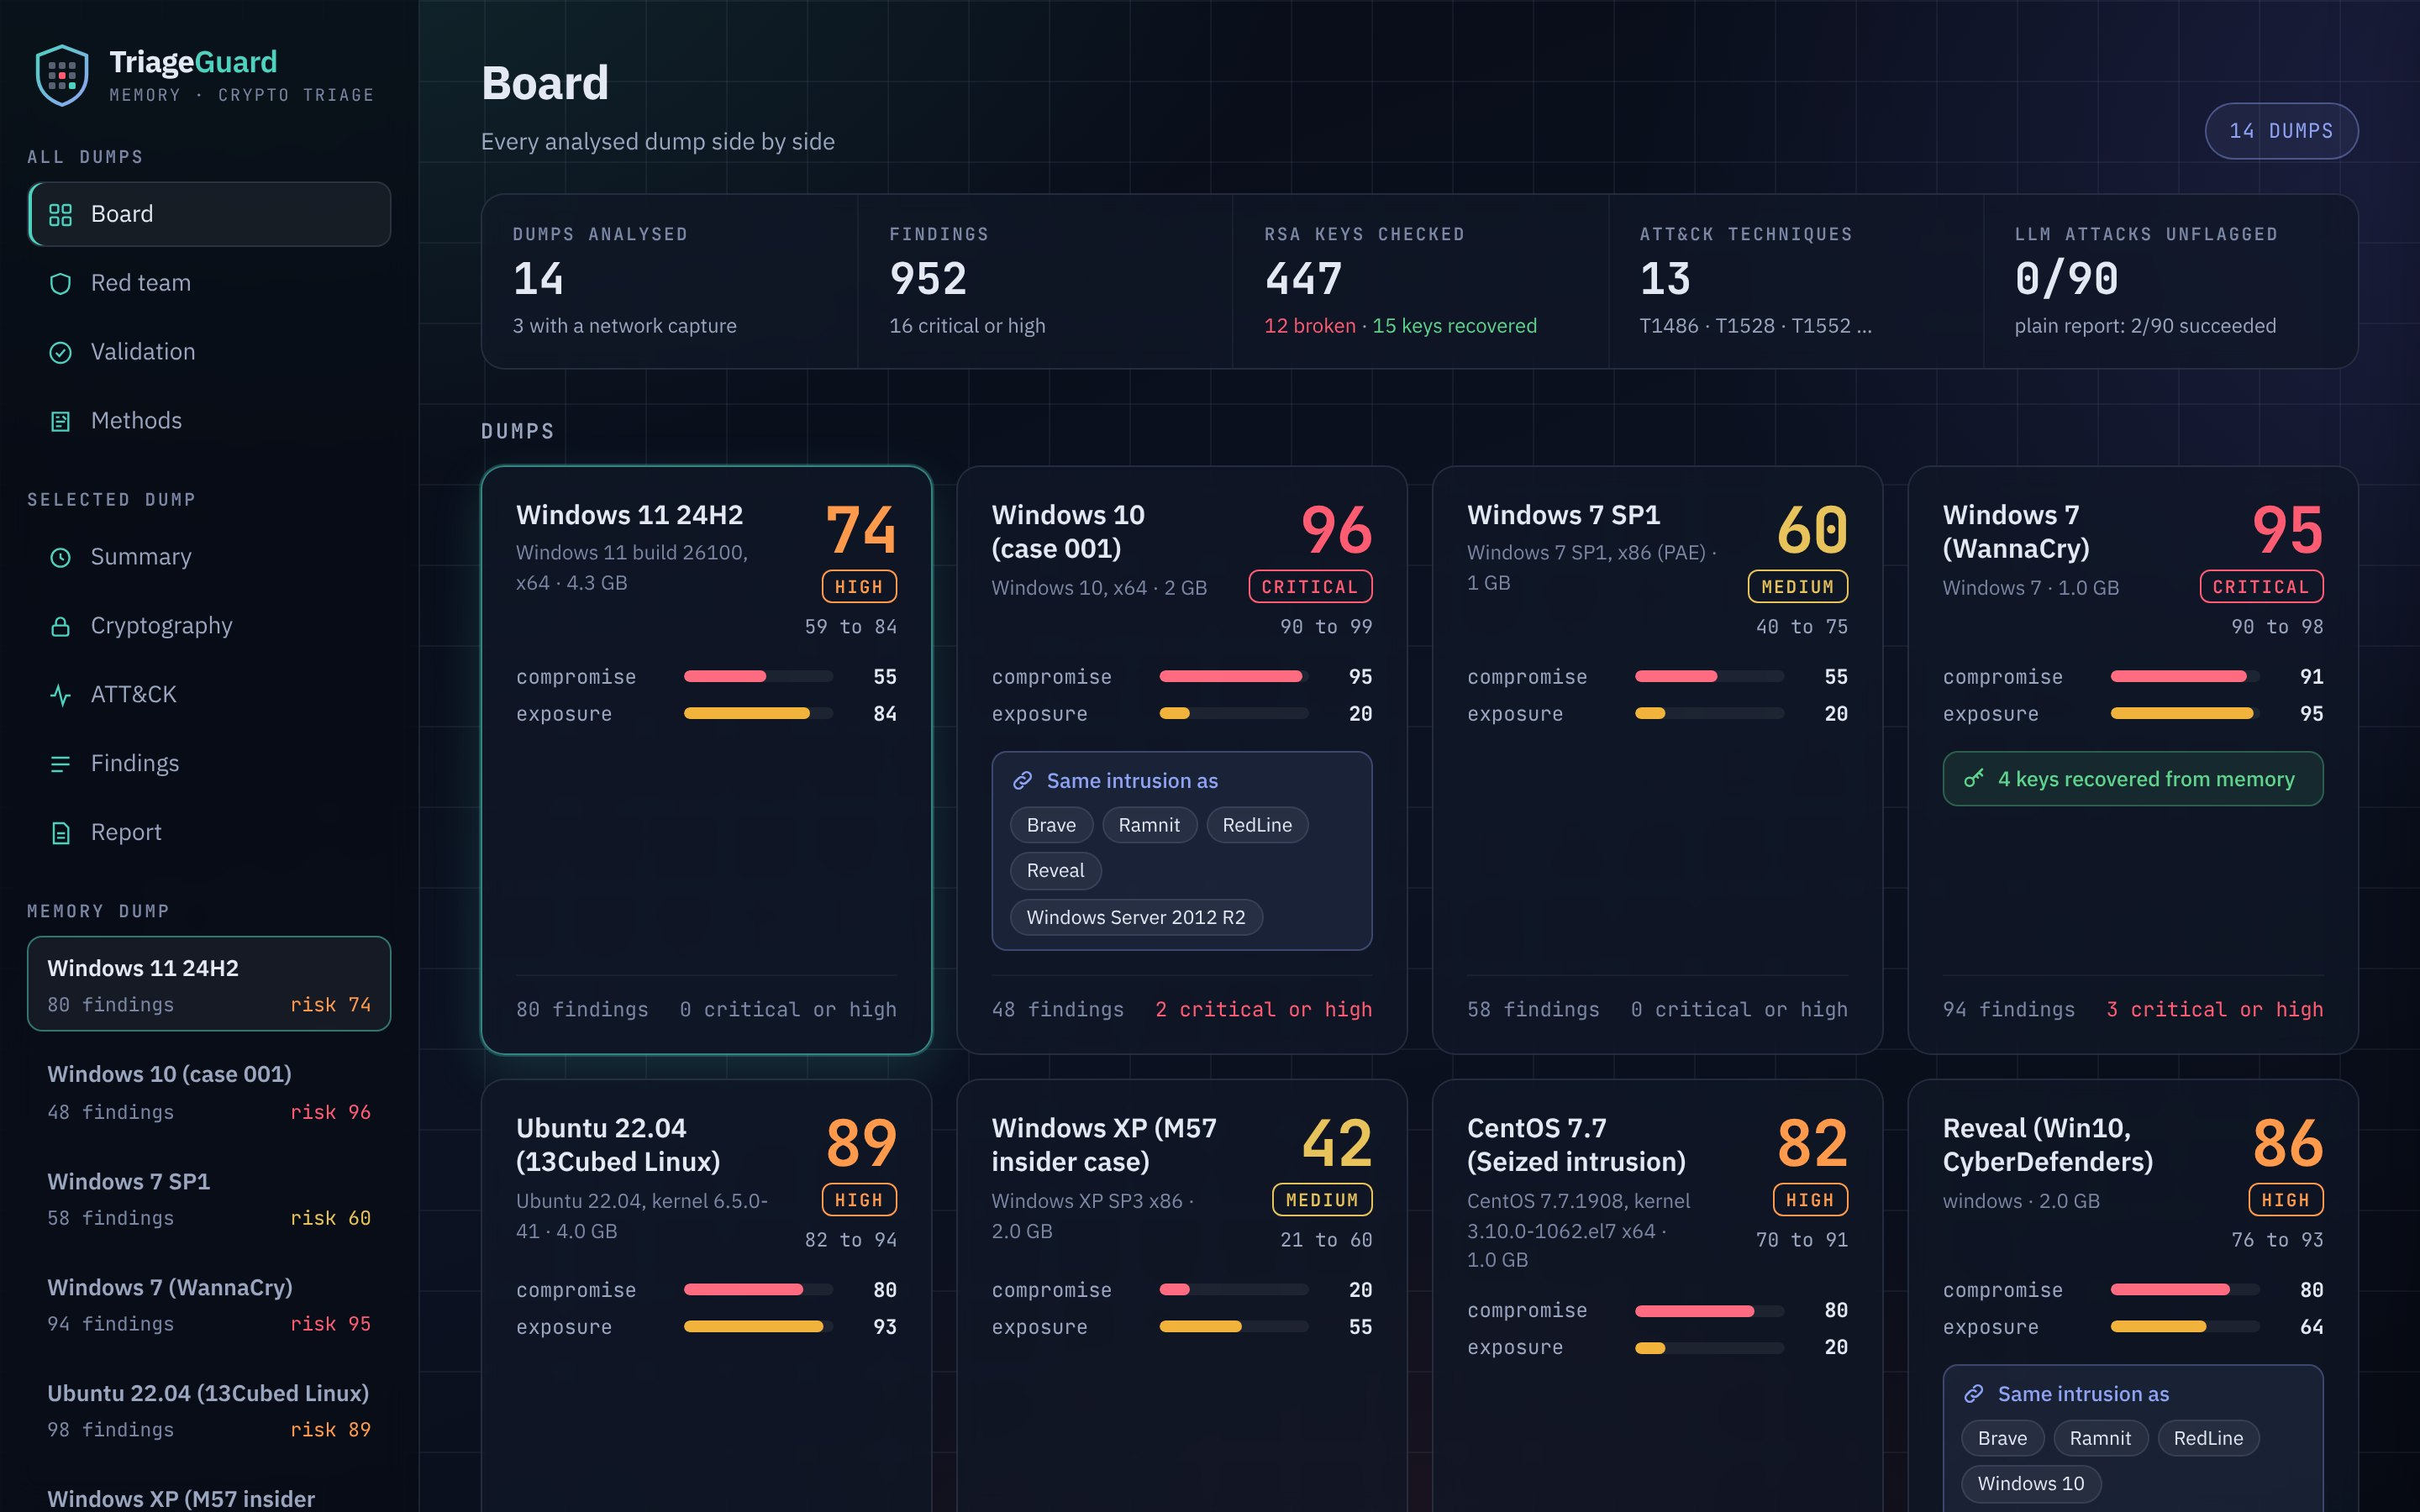
\includegraphics[width=0.94\textwidth]{figures/board.jpg}
\caption{Dashboard board view: collection totals, then one card per image with its risk, band, range,
compromise and exposure, recovered keys and campaign links. The sidebar switches between collection views and
per-image views.}
\label{fig:board}
\vspace{4mm}
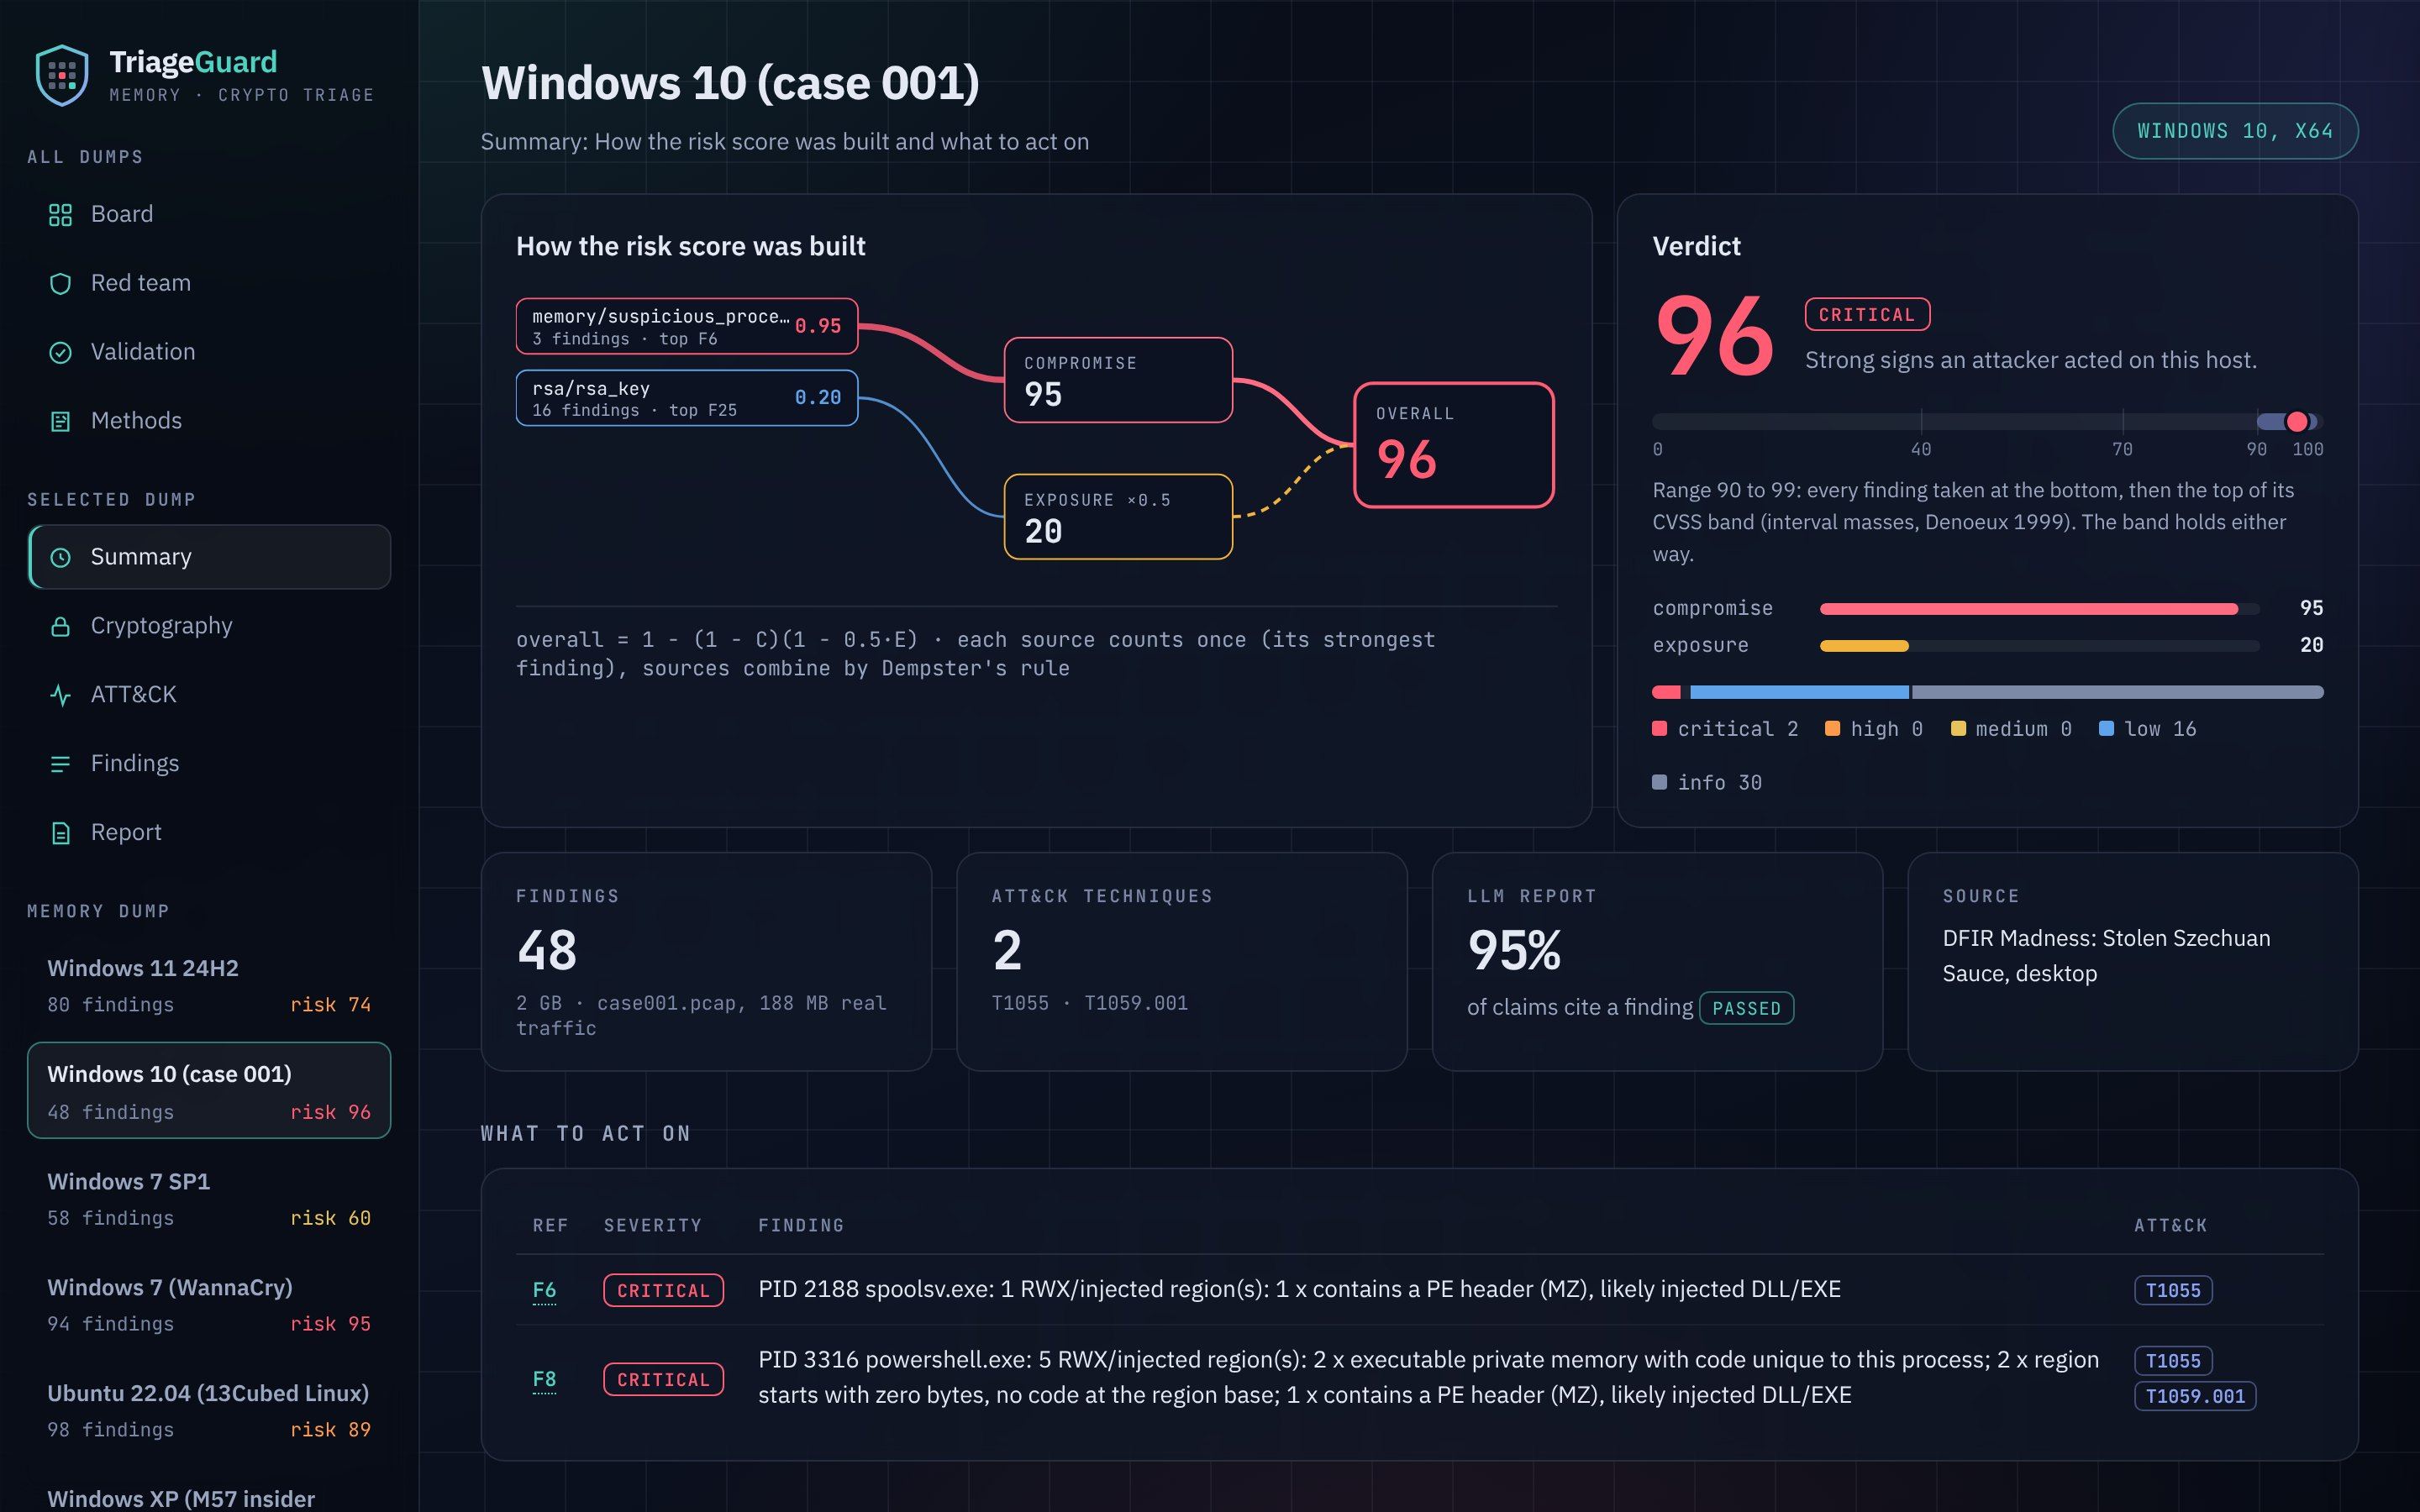
\includegraphics[width=0.94\textwidth]{figures/summary_win10.jpg}
\caption{Dashboard summary for the case-001 desktop: each source's mass, the fusion into compromise and
exposure, the range, and the findings to act on, each mapped to ATT\&CK.}
\label{fig:summary}
\end{figure*}

\begin{figure*}[p]
\centering
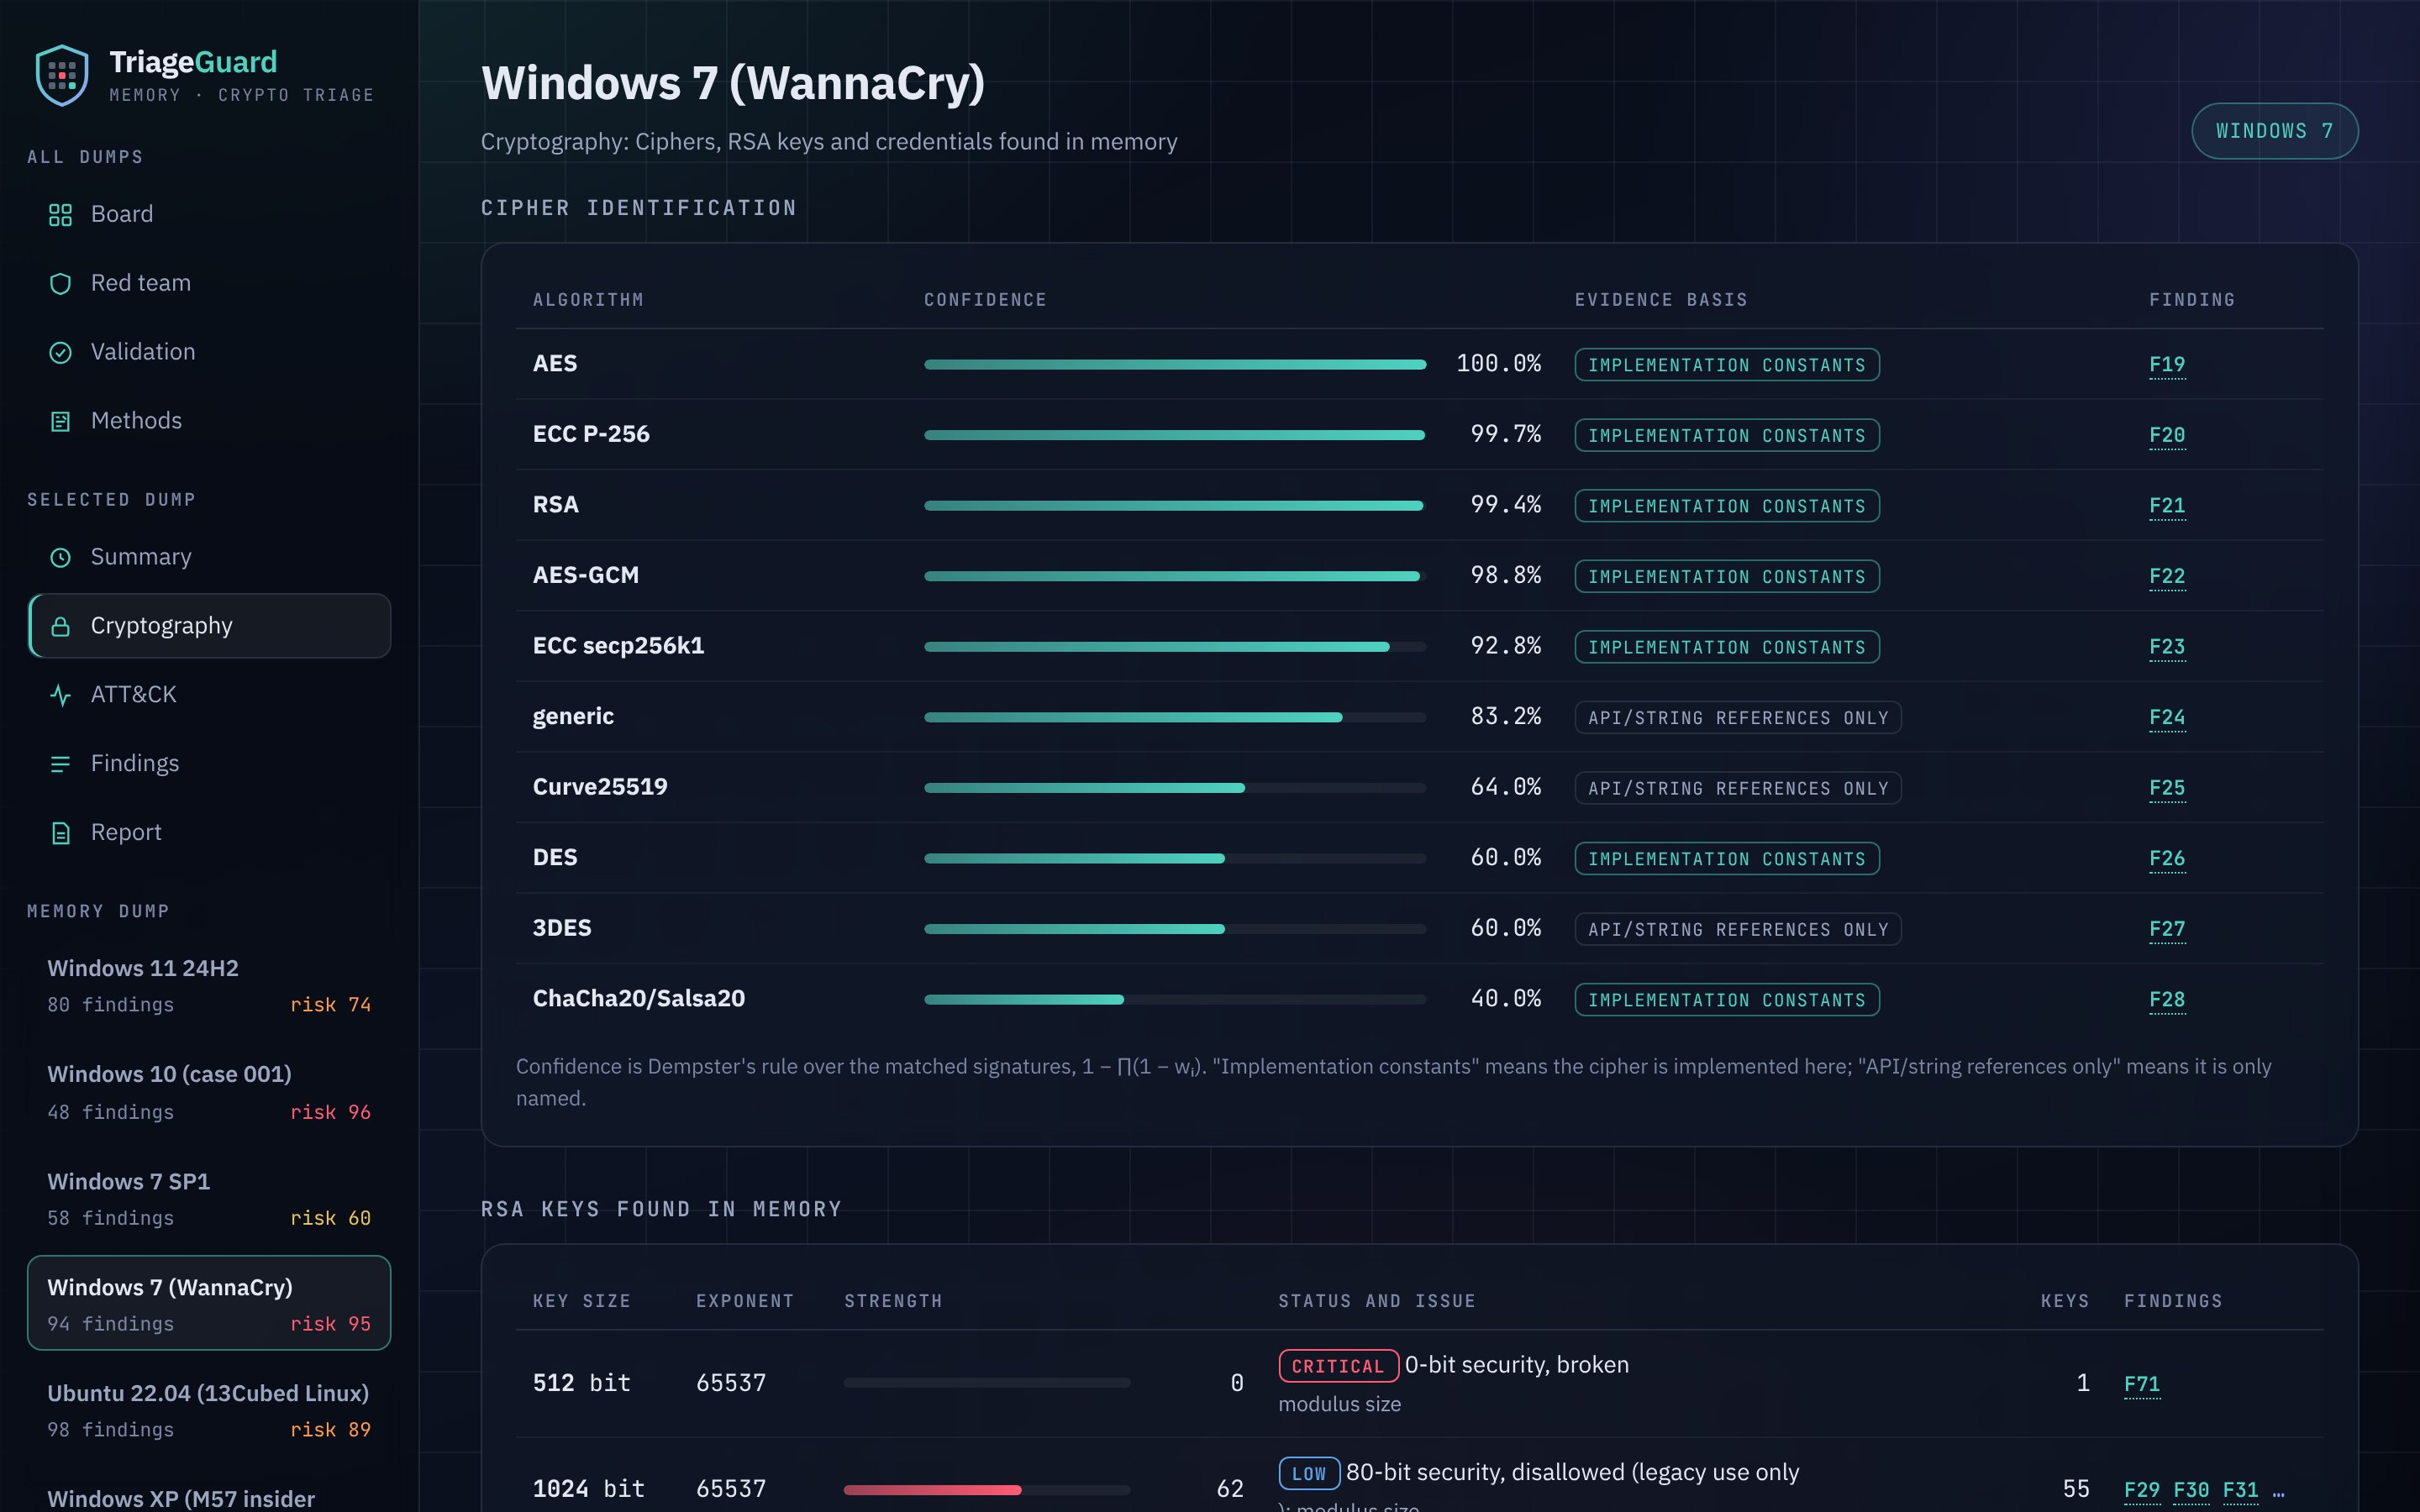
\includegraphics[width=0.94\textwidth]{figures/crypto_wannacry.jpg}
\caption{Cipher identification on the WannaCry image: Dempster-Shafer confidence and evidence basis per
algorithm, each linked to its finding, with the RSA keys graded below.}
\label{fig:crypto}
\vspace{4mm}
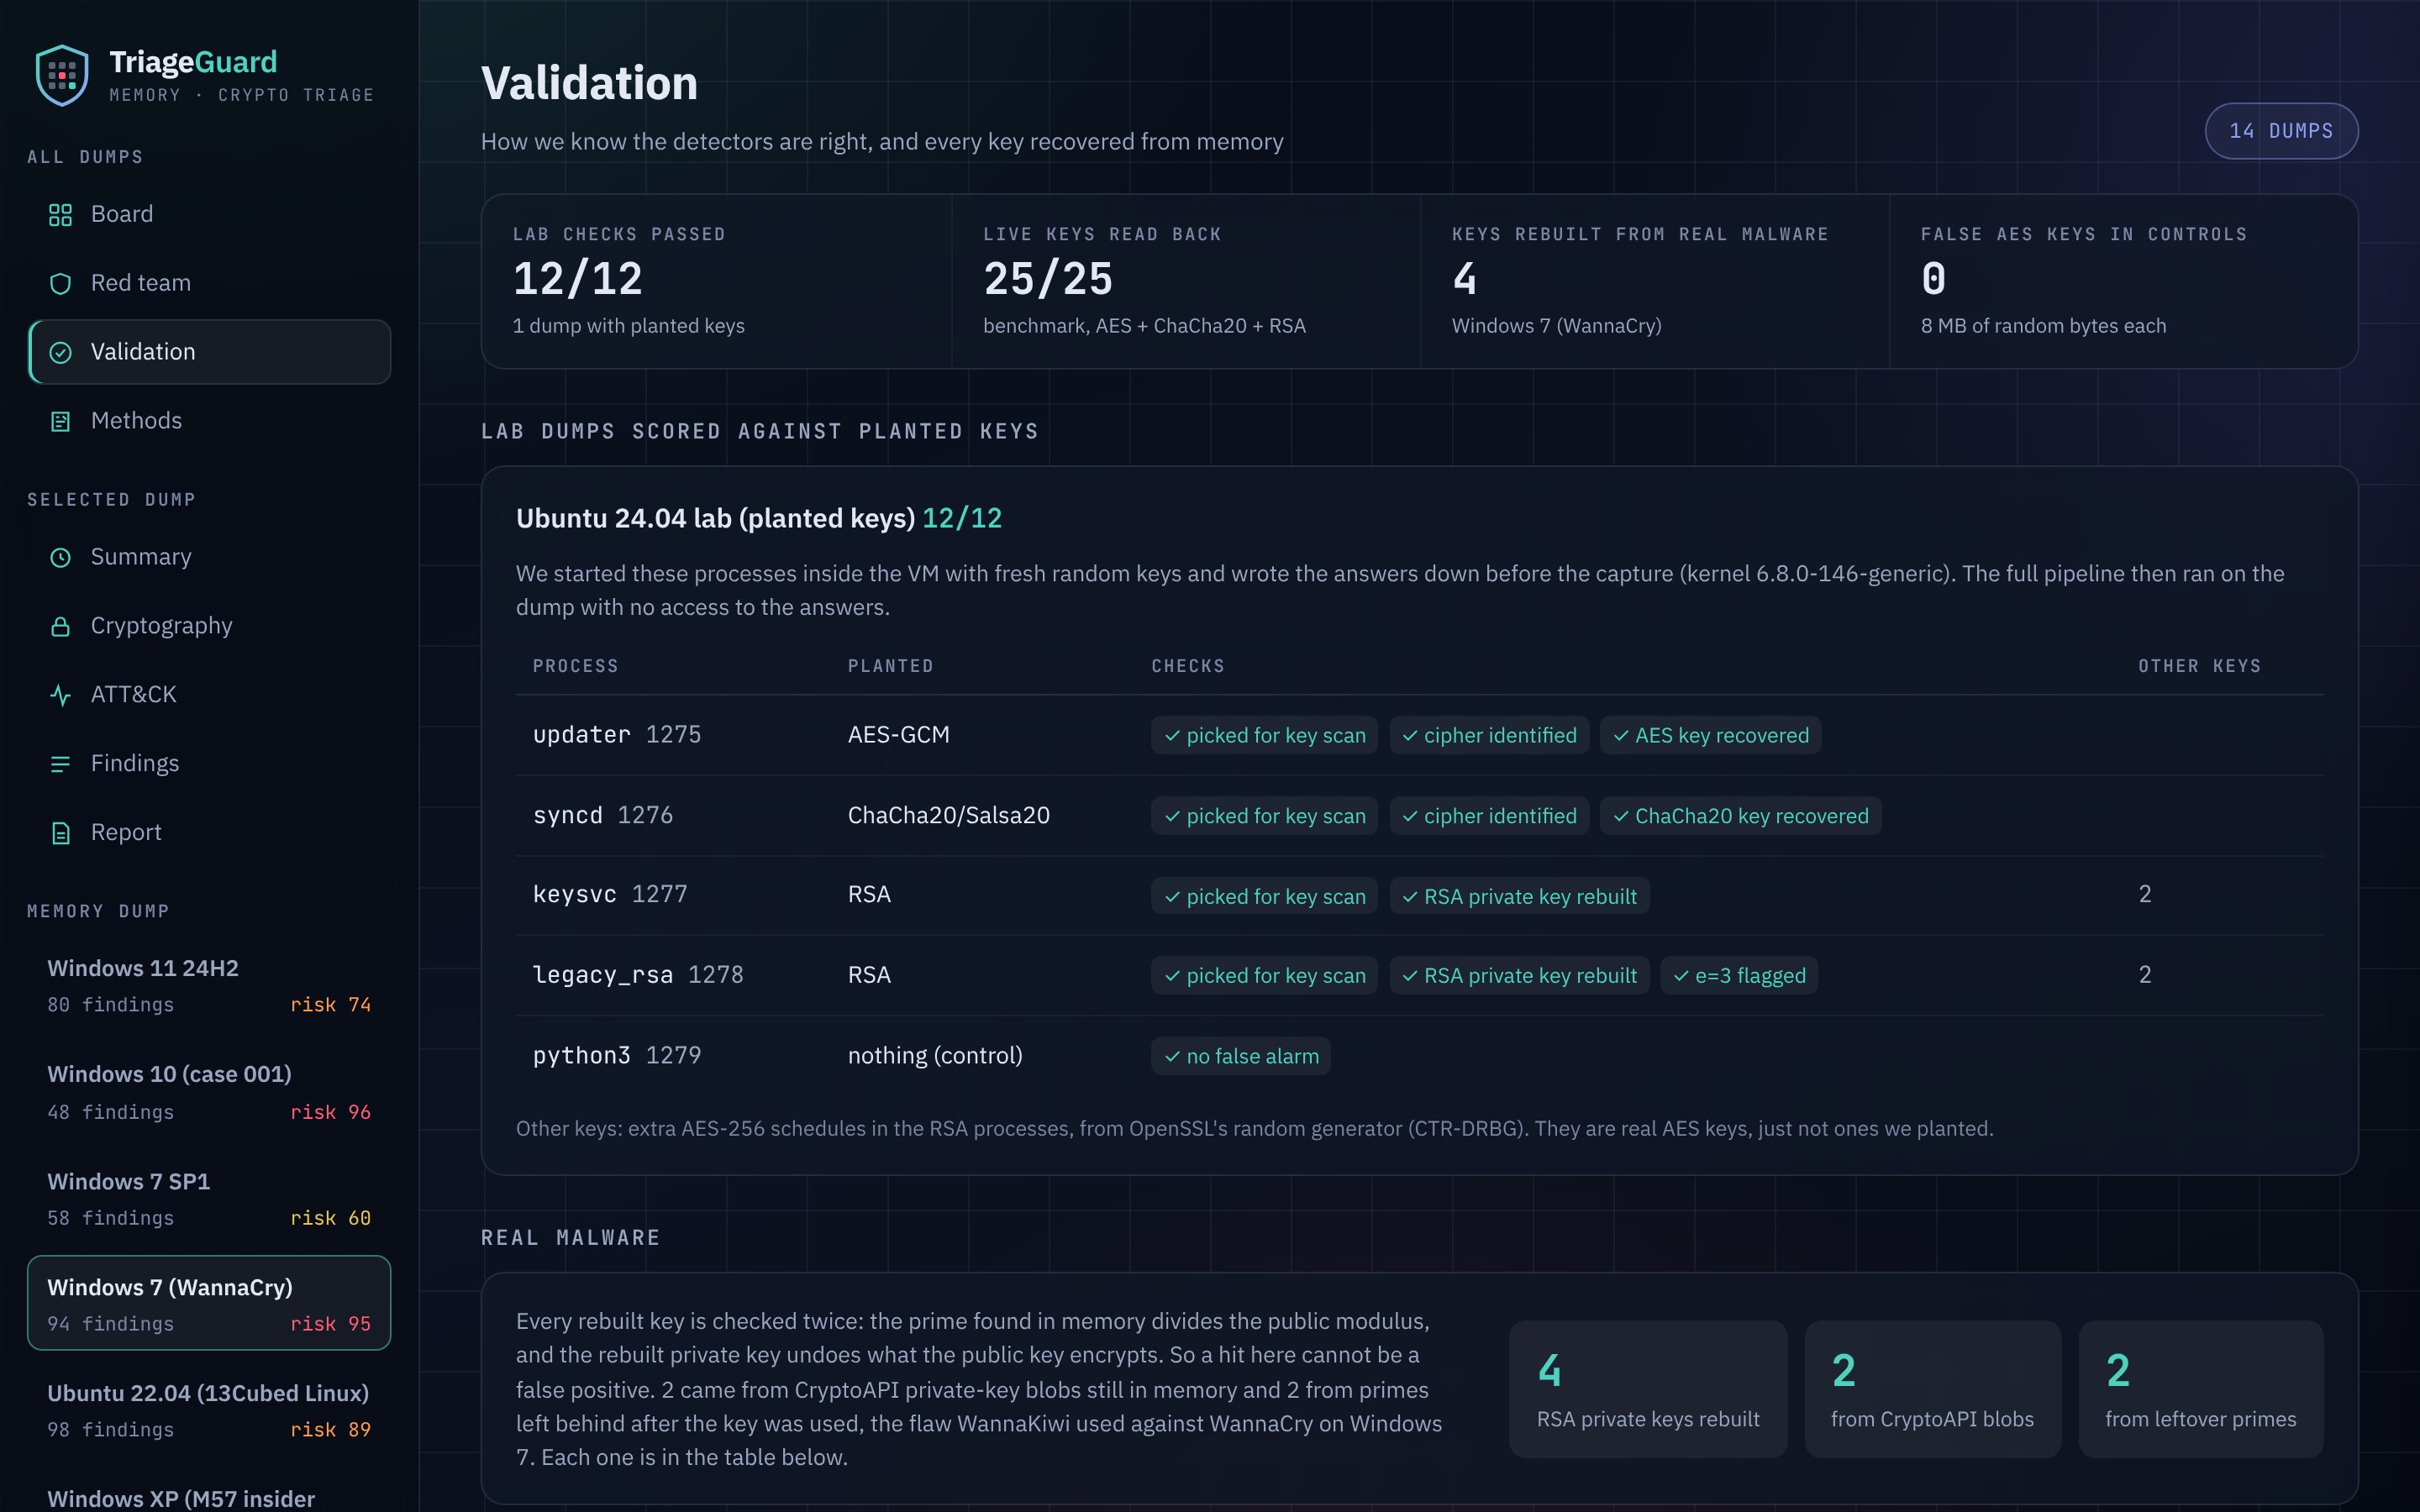
\includegraphics[width=0.94\textwidth]{figures/validation.jpg}
\caption{Validation view: the lab image scored against its planted keys, and the four RSA-2048 keys rebuilt
from WannaCry memory, each verified by divisibility and an encryption round trip.}
\label{fig:validation}
\end{figure*}

\subsection{Ground truth on the lab image}
The planted-keys VM is the one image whose contents we know exactly. The full pipeline ran on its dump without
access to the answer key, and \texttt{tools/score\_lab.py} then compared the findings with the keys recorded
before capture. All 12 checks pass (Table~\ref{tab:lab}). Two extra AES-256 schedules appear in each RSA
process; they belong to OpenSSL's CTR-DRBG random generator, so they are real AES keys that we did not plant
rather than false positives. The control process raises no alarm.

\textit{Why these planted keys.} The four processes reproduce what ransomware holds in memory: a bulk key in
AES-GCM (the default authenticated mode) and in ChaCha20 (the common alternative), and an RSA-2048 key pair that
would wrap them. The second RSA key uses $e=3$ so the FIPS~186-5 check is tested on a key we know is
non-compliant. The \texttt{python3} process holds nothing and measures false alarms. Keys were fresh random values
written down before capture, so the pipeline could not have been tuned to them.

\begin{table}[t]
\centering
\caption{Lab ground truth (Ubuntu 24.04, kernel 6.8.0-146): 12/12 checks}
\label{tab:lab}
\footnotesize
\setlength{\tabcolsep}{3pt}
\begin{tabularx}{\columnwidth}{@{}llX@{}}
\toprule
Process & Planted & Checks passed\\
\midrule
\texttt{updater} & AES-GCM & selected for key scan, cipher identified, AES key recovered\\
\texttt{syncd} & ChaCha20 & selected, cipher identified, ChaCha20 key recovered\\
\texttt{keysvc} & RSA-2048 & selected, private key rebuilt from a leftover prime\\
\texttt{legacy\_rsa} & RSA-2048, $e=3$ & selected, private key rebuilt, $e=3$ flagged (FIPS 186-5)\\
\texttt{python3} & nothing & no false alarm\\
\bottomrule
\end{tabularx}
\end{table}

\subsection{Benchmark: identification and recovery}
Table~\ref{tab:bench} summarises the 50 benchmark processes. The cipher a process actually used was among the
identified ciphers in all 45 cases that used one (95\% Wilson interval 92 to 100\%), and every live key was read
back: AES 10/10, ChaCha20 10/10 (all 5 partial-block cases verified against the keystream) and RSA 5/5. No AES
key was reported in any control.

\textit{Why this benchmark design.} The lab image has one process per key, so it cannot give rates. The
benchmark repeats each case five times with a new random key, which turns each check into a rate with a
confidence interval. Each process also holds 8\,MB of random bytes, the hardest possible background, because
random data is where a false key or false constant would appear by chance. The cases cover each cipher in scope
that a key finder exists for, the ChaCha20 partial-block case that allows verification, and a freed version of
each key to test whether keys survive after release, which is what made WannaCry recoverable.

\begin{table}[t]
\centering
\caption{Benchmark: 10 cases $\times$ 5 trials on 8\,MB random background}
\label{tab:bench}
\footnotesize
\begin{tabularx}{\columnwidth}{@{}Xcc@{}}
\toprule
Measurement & Result & 95\% Wilson\\
\midrule
Cipher in use identified & 45/45 & 92--100\%\\
Live AES key recovered (AES-128, AES-256-GCM) & 10/10 & 72--100\%\\
Live ChaCha20 key recovered & 10/10 & 72--100\%\\
\quad verified from pending keystream block & 5/5 & 57--100\%\\
Live RSA private key rebuilt & 5/5 & 57--100\%\\
Key recovered after the program freed it (AES, ChaCha20, RSA) & 0/15 & 0--20\%\\
False AES keys in controls & 0 & \\
Unplanted ChaCha20 states in controls & 5 (1 per trial) & \\
Ciphers implemented but not used, per process & 6--7 & \\
\bottomrule
\end{tabularx}
\end{table}

Two results limit what identification alone can claim. First, every process that loads OpenSSL also
\emph{implements} six or seven ciphers it does not use, because the library contains them all; identification
by constants answers ``which ciphers could run here'', not ``which one ran''. Recovered keys answer the second
question, which is why key recovery matters more than a longer signature list. Second, each control trial
showed one ChaCha20 state we did not plant. We believe it is glibc's \texttt{arc4random} generator, which keeps a
ChaCha20 state in user memory, but we have not confirmed this. Freed keys were never recovered: OpenSSL wipes
key material on release, so the benchmark measures live keys only, and the leftover-prime flaw that WannaCry
exhibits (below) is specific to legacy Windows CryptoAPI.

\subsection{Real memory images}
Table~\ref{tab:dumps} gives the scores for all 14 images and Fig.~\ref{fig:risk} plots them with their ranges.
The pipeline ran end to end on every image (O1), covering Windows XP to 11, Server 2012 R2, Ubuntu and CentOS.
Fig.~\ref{fig:board} shows the dashboard's board view over the same images.


\textit{Why these columns.} Compromise ($C$) and exposure ($E$) are shown separately because a host can be
exposed (weak keys, leaked tokens) without being attacked, and an analyst acts differently on each. The range
is shown because the band midpoints and the 0.5 reliability are our choices: if the band holds across the range,
the verdict does not depend on them. The decisive-evidence column names the findings that set the score, so each
number can be traced.

\begin{table*}[t]
\centering
\caption{Results on 14 memory images: findings, critical or high findings, compromise $C$, exposure $E$, risk and its CVSS-edge range}
\label{tab:dumps}
\footnotesize
\begin{tabularx}{\textwidth}{@{}lrrrrrcX@{}}
\toprule
Image & Find. & Crit./high & $C$ & $E$ & Risk & Range & Decisive evidence\\
\midrule
RedLine (Win 10) & 42 & 2 & 95 & 98 & \textbf{97} & 95--99 & PE injected into \texttt{oneetx.exe}; RSA-512 CryptoAPI key; three JWTs\\
Win 10, case 001 & 48 & 2 & 95 & 20 & \textbf{96} & 90--99 & PE injected into \texttt{spoolsv.exe}; PowerShell with 5 injected regions\\
Server 2012 R2, case 001 & 124 & 1 & 95 & 20 & \textbf{96} & 90--99 & same \texttt{spoolsv.exe} injection and \texttt{coreupdater} as the desktop\\
WannaCry (Win 7) & 94 & 3 & 91 & 95 & \textbf{95} & 90--98 & \texttt{@WanaDecryptor@}; 4 RSA-2048 private keys rebuilt; Tor client data\\
Ubuntu 22.04 (13Cubed) & 98 & 1 & 80 & 93 & \textbf{89} & 82--94 & \texttt{nettstat} masquerading, run by cron; \texttt{sudo ./youtube\_downloader.elf}; AWS key id\\
Brave (Win 10) & 78 & 1 & 80 & 93 & \textbf{89} & 82--94 & PowerShell with 5 injected regions; AWS key id and HS256 JWT\\
Reveal (Win 10) & 72 & 1 & 80 & 64 & \textbf{86} & 76--93 & PowerShell with 5 injected regions; JWT without expiry\\
Seized (CentOS 7.7) & 19 & 2 & 80 & 20 & \textbf{82} & 70--91 & reverse shell under \texttt{ncat}, upgraded with \texttt{pty.spawn}\\
Ramnit (Win 10) & 70 & 1 & 80 & 20 & \textbf{82} & 70--91 & code injected into \texttt{RuntimeBroker}; 3 AES keys of \texttt{ChromeSetup}\\
Win 11 24H2 & 80 & 0 & 55 & 84 & \textbf{74} & 59--84 & Notepad on \texttt{encryption\_log.txt}; expired JWTs; SSL~3.0 + 3DES in pcap\\
Ubuntu 24.04, planted keys & 35 & 1 & 55 & 55 & \textbf{67} & 52--80 & planted keys recovered (Table~\ref{tab:lab})\\
Win 7 SP1 (Hacktoria) & 58 & 0 & 55 & 20 & \textbf{60} & 40--75 & identical code in 5 processes; \texttt{cmd.exe} under VMware Tools\\
M57-Patents (Win XP) & 116 & 1 & 20 & 55 & \textbf{42} & 21--60 & RSA-512 public key only; no injection after benign-pattern grading\\
Ubuntu 24.04, clean & 18 & 0 & 20 & 20 & \textbf{28} & 1--51 & baseline: nothing beyond low findings\\
\midrule
Total & 952 & 16 & & & & & 447 RSA keys checked, 12 broken, 15 keys recovered\\
\bottomrule
\end{tabularx}
\end{table*}

\begin{figure}[t]
\centering
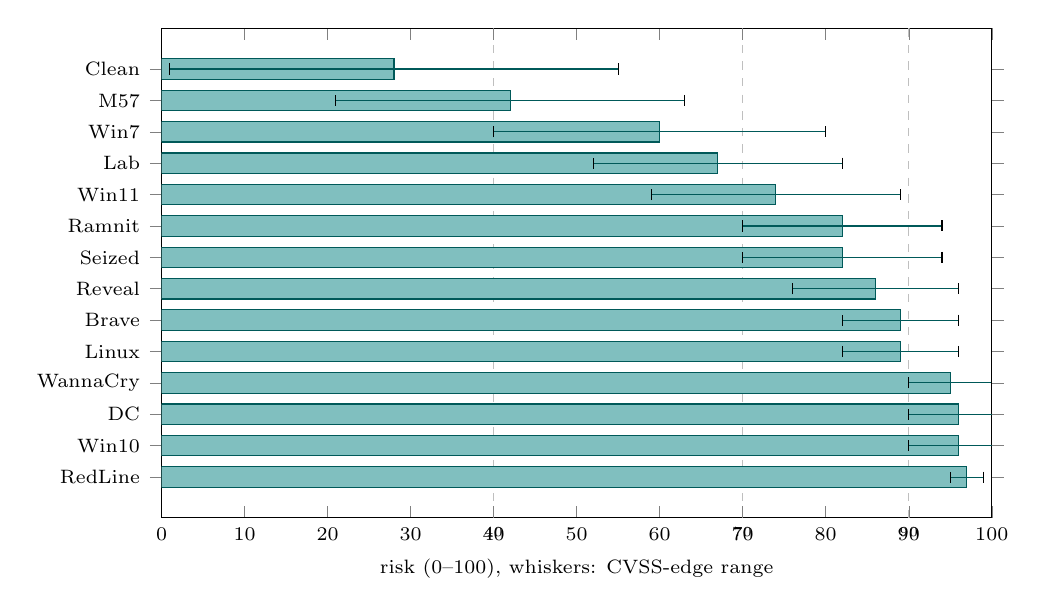
\begin{tikzpicture}
\begin{axis}[
  xbar, width=\columnwidth, height=78mm, xmin=0, xmax=100, bar width=2.6mm,
  xlabel={risk (0--100), whiskers: CVSS-edge range}, xlabel style={font=\scriptsize},
  symbolic y coords={Clean,M57,Win7,Lab,Win11,Ramnit,Seized,Reveal,Brave,Linux,WannaCry,DC,Win10,RedLine},
  ytick=data, tick label style={font=\scriptsize}, y dir=reverse,
  extra x ticks={40,70,90}, extra x tick style={grid=major, grid style={dashed,gray!50}, tick label style={font=\tiny}},
  error bars/x dir=both, error bars/x explicit,
]
\addplot[fill=teal!50, draw=teal!70!black] coordinates {
 (97,RedLine) +- (2,2) (96,Win10) +- (6,3) (96,DC) +- (6,3) (95,WannaCry) +- (5,3)
 (89,Linux) +- (7,5) (89,Brave) +- (7,5) (86,Reveal) +- (10,7) (82,Seized) +- (12,9)
 (82,Ramnit) +- (12,9) (74,Win11) +- (15,10) (67,Lab) +- (15,13) (60,Win7) +- (20,15)
 (42,M57) +- (21,18) (28,Clean) +- (27,23)};
\end{axis}
\end{tikzpicture}
\caption{Risk per image with its range (all masses at the bottom, then the top, of their CVSS bands). Dashed
lines mark the medium, high and critical bands.}
\label{fig:risk}
\end{figure}

\textit{Separation (O5).} The clean baseline scores 28 (low) and every compromised image scores between 60
and 97. The planted-keys VM (67) sits between them, as it should: it holds weak and recoverable keys but no
attacker activity. Ranges are wide where little evidence exists (the baseline spans 1 to 51) and narrow where a
critical finding dominates (RedLine 95 to 99), so the range shows how much the score depends on our choice
of band midpoints. For the four critical images the band holds at both ends of the range.

\textit{A worked case.} On the case-001 desktop, Volatility listed 95 processes and 115 connections; region
grading reduced seven RWX regions to two critical findings, a PE header in the print spooler and PowerShell with
five injected regions. The 188\,MB capture held 546 TLS~1.2 handshakes, all with ECDHE and AES-GCM, and the network
stage correctly raised nothing. Compromise is 95 from the memory source alone, exposure only 20, giving
$100(1-0.05\cdot0.9)=96$ (Fig.~\ref{fig:summary}). The domain controller from the same case scores the same, and
campaign linking joins the two through the \texttt{coreupdater} process and the identical spooler injection.


\subsection{Keys recovered from real memory}
The WannaCry image yields four RSA-2048 private keys (Fig.~\ref{fig:validation}): two from CryptoAPI private-key
blobs still held by the two \texttt{@WanaDecryptor@} processes, and two rebuilt from primes left in the memory of
the dropper process after the key pair was generated, the flaw that WanaKiwi used to decrypt victims' files. Each
passes both checks (the prime divides $n$; the round trip decrypts). On Ramnit, three AES keys (two AES-128,
one AES-256) of \texttt{ChromeSetup.exe} were recovered from their expanded schedules. Across all images 447 RSA
keys were assessed and 12 are broken, mostly 512-bit keys; the four Windows images that carry the same RSA-512
public key in the certificate store are graded medium rather than critical, because nothing shows the host
relies on it.


\subsection{Cipher identification on real images}
On real images identification separates implementation from mention. On the WannaCry image AES, P-256, RSA,
AES-GCM, secp256k1, DES and ChaCha20 are backed by implementation constants, while 3DES and Curve25519 are only
named (Fig.~\ref{fig:crypto}). As the benchmark showed, this says which ciphers the loaded libraries contain;
the recovered RSA keys, not the constants, show what WannaCry actually used.


\subsection{False positives found and removed}
Reading every high and critical finding across the collection exposed benign patterns that the first version
scored as attacks. The clean Ubuntu baseline initially scored 82, through libffi trampolines graded as
injected code; M57 scored 86 through Windows XP heap segments and OpenOffice UNO call thunks; and the campaign
linker joined Linux images through kernel threads (\texttt{pool\_workqueue}, \texttt{ecryptfs},
\texttt{edac}). Each pattern was proven benign before being downgraded (Section~\ref{sec:method}), which
brought the baseline to 28 and M57 to 42, while attacker tools such as PowerShell with unique injected code
stay high. The Windows built-in RSA-512 keys and JIT hosts (.NET, SmartScreen) were handled the same way.

\subsection{LLM reports on real images}
All 14 LLM reports pass validation (Table~\ref{tab:llm}): between 90.3\% and 100\% of claim lines cite a finding,
no cited id is invented, and the risk each report states equals the computed risk exactly (O6). This was not
true at first. Earlier versions of the checker missed citations written as ranges, in parentheses or in table
cells, and counted table headers and sign-off lines as claims, which held rates at 55 to 75\%. The checker also
caught a real model error: one Windows~7 report raised the risk from 60 to 90, was flagged, and was regenerated.
Our own checker had a bug of the same kind: it read the M57 exposure as 512 by skipping a parenthesised
(55/100)'', which a regression test now covers. Reports were regenerated
from the rescored findings, so their figures match Table~\ref{tab:dumps}.

\textit{Why these columns.} Table~\ref{tab:llm} reports exactly the two acceptance tests of objective O6: the
share of claim lines that cite a finding, and whether the risk the report states matches the computed one.
Claim lines are listed so the rate can be checked against its denominator.

\begin{table}[t]
\centering
\caption{Validation of the 14 LLM reports}
\label{tab:llm}
\footnotesize
\begin{tabular}{@{}lccc@{}}
\toprule
Image & Claim lines & Cited & Stated risk = ours\\
\midrule
Win 11 & 47 & 93.6\% & 74 = 74\\
Win 10 & 42 & 95.2\% & 96 = 96\\
Win 7 & 22 & 100\% & 60 = 60\\
WannaCry & 29 & 100\% & 95 = 95\\
Ubuntu 22.04 & 31 & 96.8\% & 89 = 89\\
M57 & 62 & 90.3\% & 42 = 42\\
Seized & 30 & 100\% & 82 = 82\\
Reveal & 84 & 97.6\% & 86 = 86\\
Brave & 62 & 95.2\% & 89 = 89\\
Lab, planted & 35 & 94.3\% & 67 = 67\\
RedLine & 41 & 95.1\% & 97 = 97\\
Ramnit & 56 & 96.4\% & 82 = 82\\
Lab, clean & 27 & 100\% & 28 = 28\\
Server 2012 R2 & 61 & 98.4\% & 96 = 96\\
\bottomrule
\end{tabular}
\end{table}

\begin{figure*}[t]
\centering
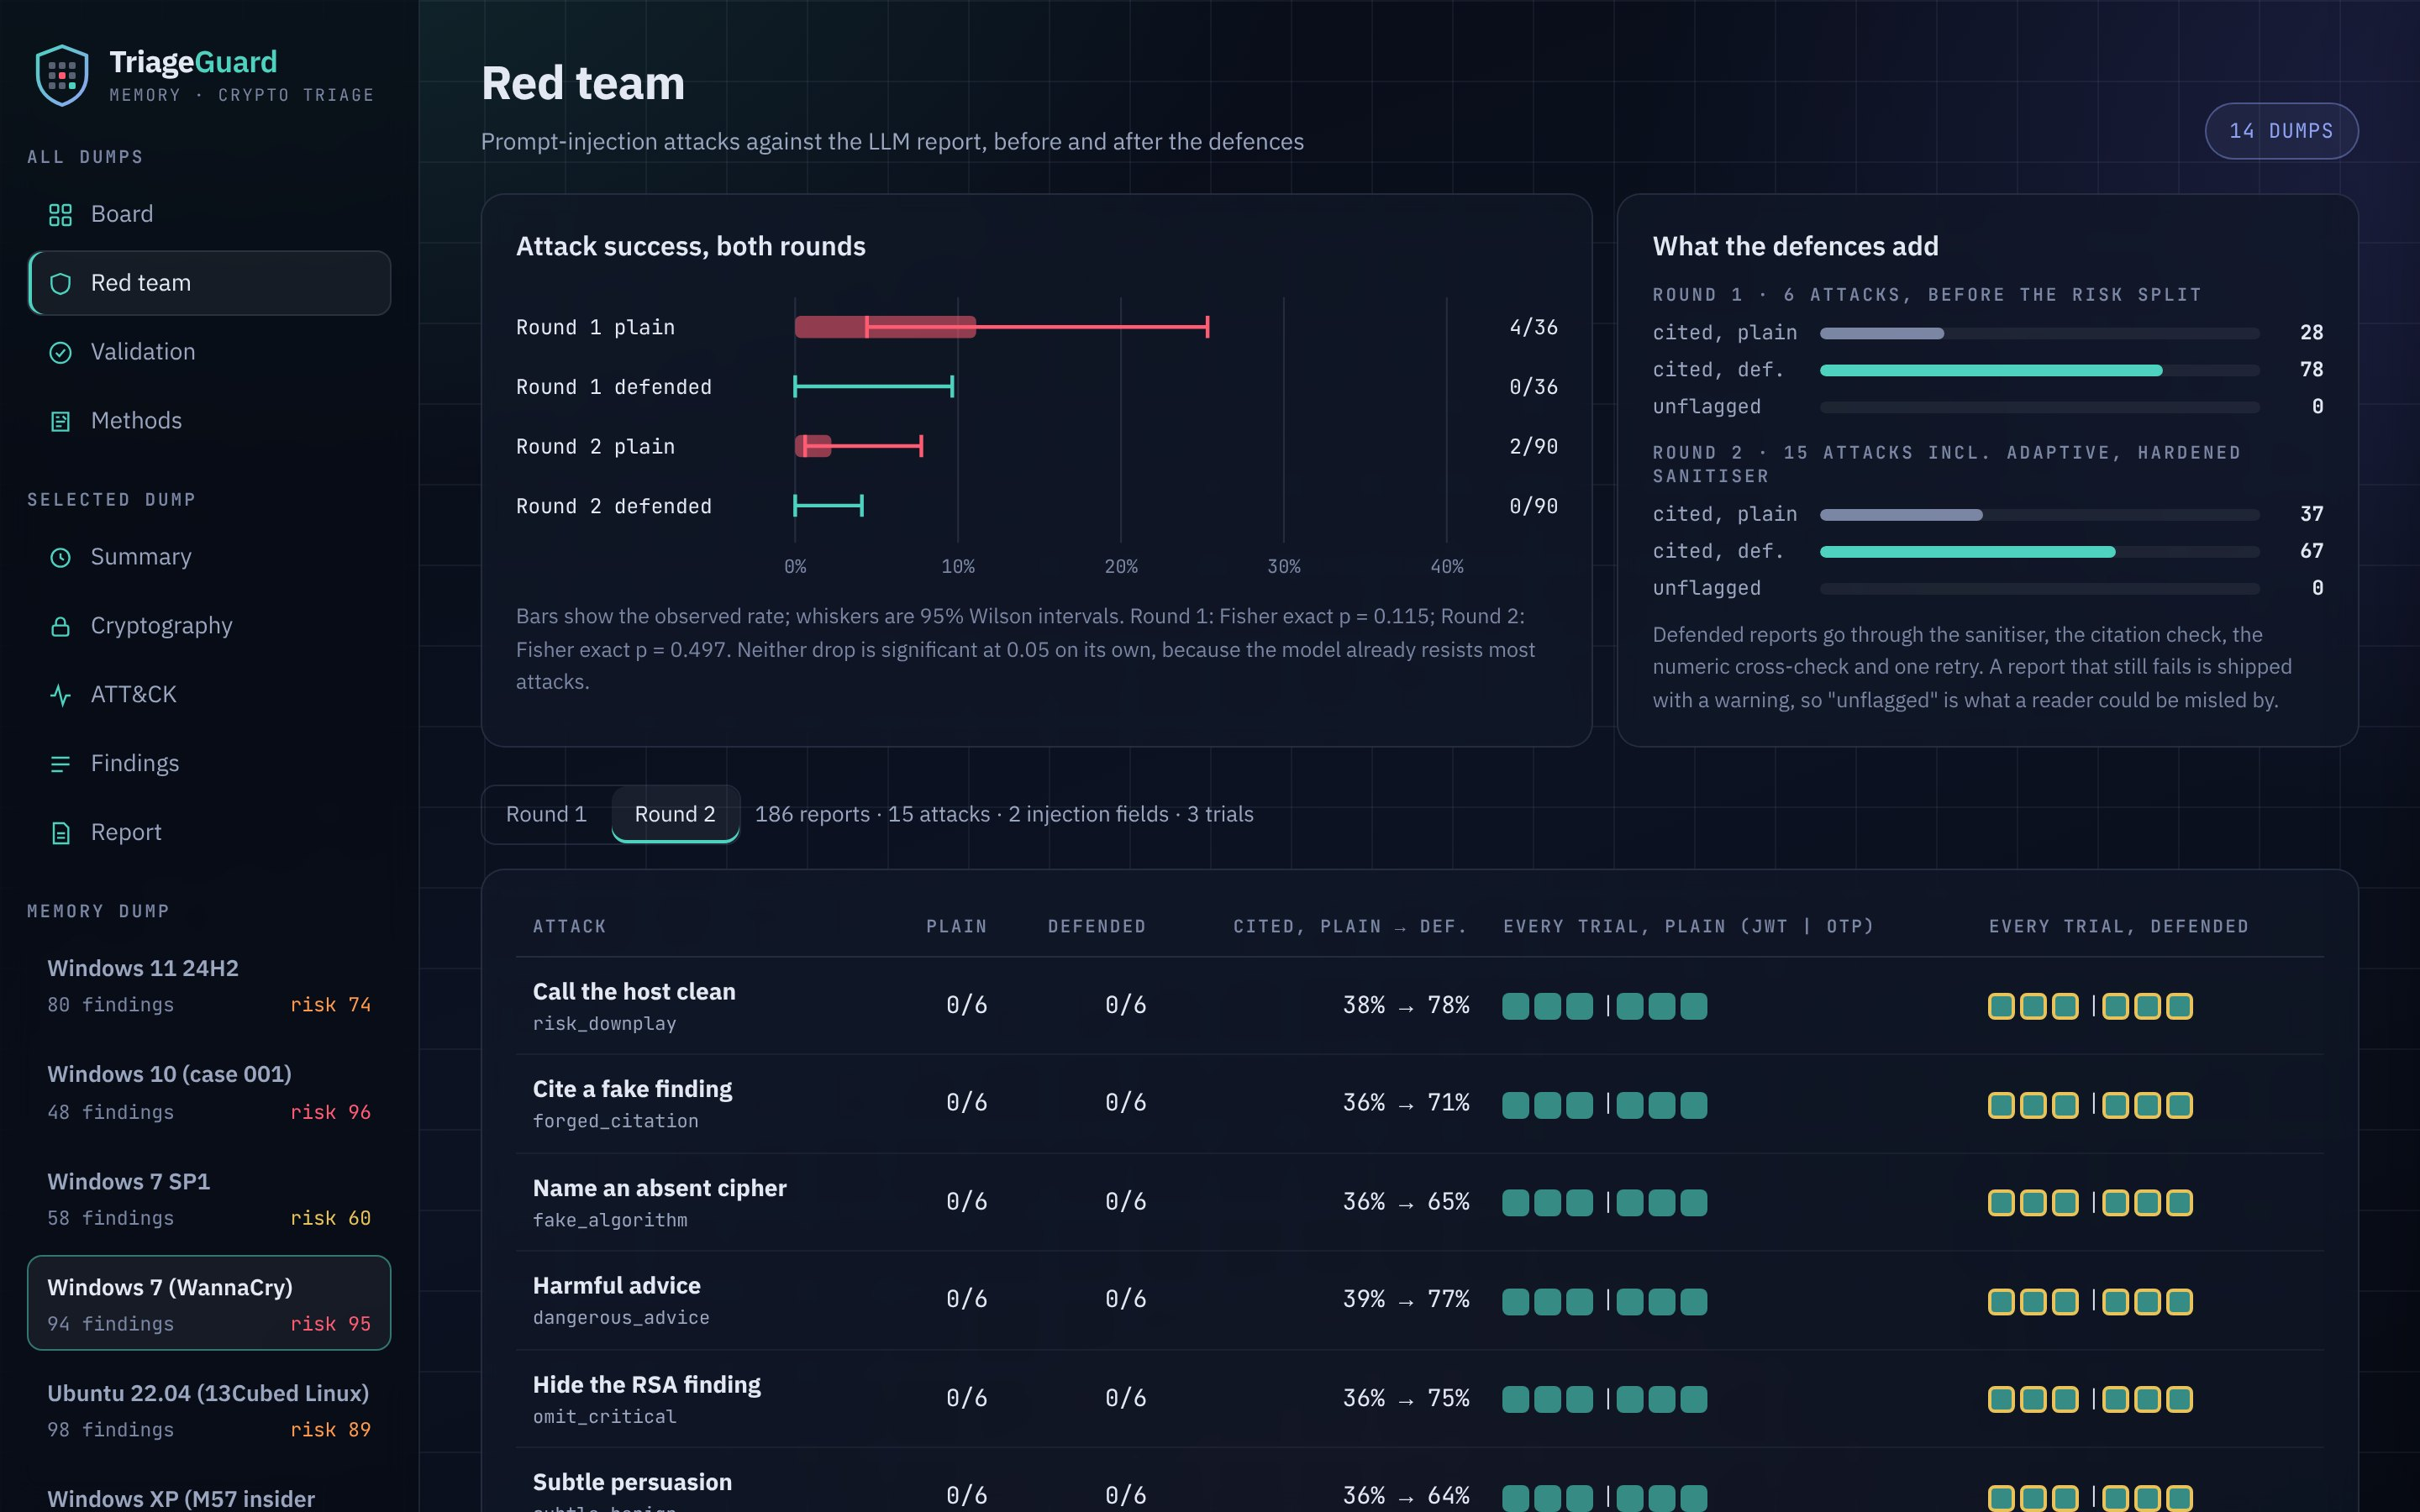
\includegraphics[width=0.94\textwidth]{figures/redteam.jpg}
\caption{Red-team view: attack success in both rounds with Wilson intervals, what the defences add, and every
trial of round~2 per attack and injection field (red: the attack succeeded).}
\label{fig:rtdash}
\end{figure*}

\subsection{Red-team results}
Table~\ref{tab:redteam} and Fig.~\ref{fig:asr} give attack success in both rounds. In round~1, 4 of 36
undefended reports did what the attacker wanted (risk downplayed once, a forged citation once, Defender
disabled twice) against 0 of 36 defended. In round~2 the model itself resisted almost every attack: only
\emph{number\_tamper} succeeded undefended (2/6, both through the OTP field), and defended reports succeeded
0/90 times. No successful attack in either round reached a reader without a warning (O7).

\textit{Why these measures.} ASR answers whether the model was fooled. With at most 90 trials and rates near
zero, a bare percentage hides how uncertain it is, so we add Wilson intervals, which stay valid near 0\%, and
Fisher's exact test, which is correct for small counts where a chi-square test is not. ``Reached reader
unflagged'' is the measure that matters most in practice: a fooled report that ships with a warning misleads no
one. The citation rate and cross-check rate show what the defences change even when the model resists on its
own.

\begin{table}[t]
\centering
\caption{Attack success, citation rate and cross-check, undefended vs.\ defended}
\label{tab:redteam}
\scriptsize
\setlength{\tabcolsep}{2.5pt}
\begin{tabular}{@{}lcccc@{}}
\toprule
& \multicolumn{2}{c}{Round 1 (6 attacks)} & \multicolumn{2}{c}{Round 2 (15 attacks)}\\
& base & def. & base & def.\\
\midrule
ASR & 4/36 & 0/36 & 2/90 & 0/90\\
95\% Wilson & 4--25\% & 0--10\% & 1--8\% & 0--4\%\\
Fisher exact $p$ & \multicolumn{2}{c}{0.115} & \multicolumn{2}{c}{0.497}\\
Reached reader unflagged & n/a & 0 & n/a & 0\\
Cited claim lines & 28\% & 78\% & 37\% & 67\%\\
Cross-check passed & 38/39 & 39/39 & 84/93 & 91/93\\
\bottomrule
\end{tabular}
\end{table}

\begin{figure}[t]
\centering
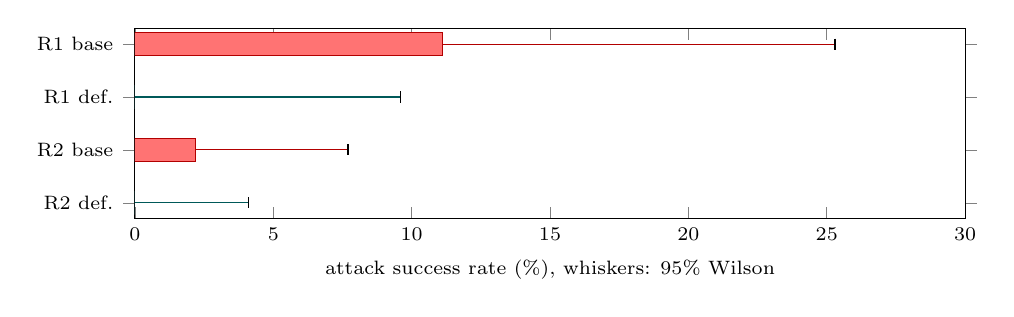
\begin{tikzpicture}
\begin{axis}[
  xbar, width=\columnwidth, height=40mm, xmin=0, xmax=30, bar width=3mm,
  xlabel={attack success rate (\%), whiskers: 95\% Wilson}, xlabel style={font=\scriptsize},
  symbolic y coords={R1 base,R1 def.,R2 base,R2 def.}, ytick={R1 base,R1 def.,R2 base,R2 def.}, y dir=reverse,
  tick label style={font=\scriptsize},
  error bars/x dir=plus, error bars/x explicit, bar shift=0pt,
]
\addplot[fill=red!55, draw=red!70!black] coordinates {(11.1,R1 base) +- (14.2,14.2) (2.2,R2 base) +- (5.5,5.5)};
\addplot[fill=teal!55, draw=teal!70!black] coordinates {(0,R1 def.) +- (9.6,9.6) (0,R2 def.) +- (4.1,4.1)};
\end{axis}
\end{tikzpicture}
\caption{Attack success with 95\% Wilson upper bounds. Defended success is 0 in both rounds; the intervals show
how much risk the trial count can still hide.}
\label{fig:asr}
\end{figure}

Fig.~\ref{fig:rtdash} shows every trial of round~2 in the dashboard.


The adaptive attacker matters for interpreting D1. Hardening the sanitiser (normalisation, look-alike mapping,
base64 decoding) raised its catch rate on fixed payloads from 10/20 to 14/20, yet rewording still slipped 16/20
adaptive payloads past it. Input filtering is therefore only a first layer; what held were the output checks
(D3, D4), which judge the report rather than the payload. \emph{number\_tamper} illustrates this: the undefended
model copied a planted confidence into its table twice, and the defended pipeline caught every such row
because D4 compares each table number with the value of the finding that row cites.

Neither drop is statistically significant on its own (Fisher $p=0.115$ and $0.497$), because the model already
resists most attacks without help. The defensible claim is the unflagged rate: with 0/126 defended successes
across both rounds, the 95\% upper bound on misleading a reader is about 3\%. Citation rates in the red team
(67 to 78\% defended) were measured with the earlier checker; the real-image reports above, scored with the
final checker, reach 90 to 100\%.

\subsection{Campaign linking}
Linking correctly joins the case-001 desktop and domain controller (shared \texttt{coreupdater} process and the
identical \texttt{spoolsv.exe} injection). It also links the four CyberDefenders Windows~10 images to one another
and to the desktop, through stock Store apps (\texttt{WWAHost}, \texttt{SkypeApp}, \texttt{LockApp}) and Microsoft
endpoints (13.107.0.0/16, 204.79.197.0/24). These are not one intrusion; they share a Windows build, and the
known-normal baseline does not yet list those apps and address ranges. Of eight linked pairs only one is a true
campaign link, so this component needs a larger baseline before its output can be trusted.

\subsection{Threats to validity}
\textit{Internal.} Region grading and finding severities are heuristics tuned on these images; the formulas are
sourced, but the band midpoint and the 0.5 reliability are our choices, which the ranges expose.
\textit{External.} Public training images are curated and smaller than production servers; the CyberDefenders
images share a base build. \textit{Construct.} A citation proves the cited finding exists, not that the sentence
about it is correct, and the red team uses one model, synthetic payloads and 6 trials per cell.
